\documentclass[10pt]{article}
\usepackage{mathtools}
\usepackage{amsmath}
\usepackage{tabularx}
\usepackage{graphicx}

\begin{document}
\setlength\parindent{1pt}
\title{Project 1}
\author{Andrei Kukharenka and Anna Gribkovskaya \\  
FYS 4150 
}

\maketitle
\begin{abstract}
Andrei's part.
\end{abstract}
\clearpage 


\section{Introduction}
In this project we are dealing with the Poisson equation. This is a second order inhomogeneous differential equation of elliptic type. In this project we have a very simple case of equation in one dimension. We are going to discretize this equation and rewrite it in form of system of linear equations. We can then use some methods from linear algebra to find a solution. This kind of equations is common in physics. For example it can describe an electrostatic or gravitational fields.  \\* 
Below is a brief description of the project structure. \\* 
In this project we take a look at Poisson equation for electrostatic potential generated by a localized charge distribution. The mathematical details are discussed in Part 1. Problem formulation.\\* 
After we formulated the problem we consider some general and most useful methods we can use to solve it in the Part 2. Theory and methods. We are going to use linear algebra methods for the problem. A short description of the Gaussian elimination and LU decomposition will be given there, as well as some discussion of the pros and cons for each of them.\\* 
In Part 3. the results are presented. We took the most interesting (to our point of view) data and present it in tables and graphs. \\* 
The next part is discussion of the results. Here we evaluate our results as well as methods used to obtain them. \\* 
The last part of the report is Conclusion. Here we sum up all said above and come up with the possible topics for the further studies  in this topic. 

\section{Problem formulation}
The problem we deal with is a second order differential equation (DE) with inhomogenious term. Generally it can be written in a following form:
\[
\frac{d^2y}{dx^2}+k^2(x)y = f(x),
\]
where $y$ is unknown function of $x$, $f(x)$ is inhomogeneous term and $k^2$ is a real function.\\* 
Our DE is a classical equation of electrostatic potential, which is generated by some known charge distribution. 
\[
\nabla^2 \Phi = -4\pi \rho ({\bf r}).
\]
where $\Phi$ is electrostatic potential and $\rho ({\bf r})$ is charge distribution. \\* 
This is equation for three dimensions. We simplify this to one dimension equation in $r$ assuming the functions for electrostatic potential and charge  being spherically symmetric. After some simple variable substitution we get a general form for one-dimensional Poisson equation. We also need some boundary conditions for the equation. In this project we have a Dirichlet boundary conditions. All together it will then look as follows:
\begin{equation}\label{equ:one}
-u''(x) = f(x), \hspace{0.5cm} x\in(0,1), \hspace{0.3cm} u(0) = u(1) = 0.
\end{equation}

Here we need to introduce a disctretization of the derivative. In order to do this we first discretize a domain and define a so-called grid points for the $ x $. We have $x\rightarrow x_{i}$ and for the each of a grid points we have a discretize value of the function in this point $u(x_{i})\rightarrow v_i$. For simplisity we have the same distance between all grid point and this is so-called step lenght $ h $. Each grid poin can now be calculated as $x_i=ih$. The valuse $ h $ can be calculated as $h=1/(n+1)$. And the boundary condition is now defined as $v_0 = v_{n+1} = 0$. $ n $ is number of the steps in discretization. The discretized Poisson equation then will be
\[
   -\frac{v_{i+1}+v_{i-1}-2v_i}{h^2} = f_i  \hspace{0.5cm} \mathrm{for} \hspace{0.1cm} i=1,\dots, n,
\]

 $f_i$ here is the actual function at grid points $f(x_i)$. \\* 
 If we now run $ i $ from $ 1 $ to $ n $ it's easy to show that our discretized equation can be written as a set of linear algebra equations (SLAE):
 \\* 
  \\* 
\begin{equation}
\begin{cases}
0 - v_{1}-v_{2} = f_1h^2 \\ -v_{1}+2v_{2}-v_{3} = f_1h^2  \\ 
-v_{2}+2v_{3}-v_{4} = f_1h^2  \\ \dots  \\ -v_{n-1}+2v_{n}-0= f_1h^2 \\
\end{cases},
\end{equation}

here we use $v_0 = v_{n+1} = 0$ conditions and miultiply the right hand side of the equation with an $ h^2 $. To simplify this we now introduce a new function $\tilde{b}_i=h^2f_i$. This system can be now written in a matrix form as:
\begin{equation}\label{equ:three}
   {\bf A}{\bf v} = \tilde{{\bf b}},
\end{equation}
where ${\bf A}$ is an $n\times n$  tridiagonal matrix  
\begin{equation}
    {\bf A} = \left(\begin{array}{cccccc}
                           2& -1& 0 &\dots   & \dots &0 \\
                           -1 & 2 & -1 &0 &\dots &\dots \\
                           0&-1 &2 & -1 & 0 & \dots \\
                           & \dots   & \dots &\dots   &\dots & \dots \\
                           0&\dots   &  &-1 &2& -1 \\
                           0&\dots    &  & 0  &-1 & 2 \\
                      \end{array} \right),
\end{equation}
In our case we have a tridiagonal matrix with the same elements along the main diagonal (as well as to other diagonals). However we will look at more general case, the tridiagonal matrix with different elements along diagonals. 
\begin{equation}
    {\bf A} = \left(\begin{array}{cccccc}
                           b_1& c_1 & 0 &\dots   & \dots &\dots \\
                           a_1 & b_2 & c_2 &\dots &\dots &\dots \\
                           & a_2 & b_3 & c_3 & \dots & \dots \\
                           & \dots   & \dots &\dots   &\dots & \dots \\
                           &   &  &a_{n-2}  &b_{n-1}& c_{n-1} \\
                           &    &  &   &a_{n-1} & b_n \\
                      \end{array} \right)\left(\begin{array}{c}
                           v_1\\
                           v_2\\
                           \dots \\
                          \dots  \\
                          \dots \\
                           v_n\\
                      \end{array} \right)
  =\left(\begin{array}{c}
                           \tilde{b}_1\\
                           \tilde{b}_2\\
                           \dots \\
                           \dots \\
                          \dots \\
                           \tilde{b}_n\\
                      \end{array} \right).
\end{equation}
This kind of SLAE can be solved using different linear algebra methods. In the next section we will discuss some of them.
\section{Theory and methods}
\subsection{Gaussian elimination (GE)} 
When we have a SLAE formulated as in (3), we would like to change the matrix $ A $ so it become all zeroes below the diagonal. The most straightforward way to do it is Gauss elimination. \\*
The algorithm for the Gaussian elimination can be described as to main operations the forward substitution and the backward substitution. In t	he first part, the forward substitution, we would transform the original matrix $ A $ to some other matrix, with zeroes below the main diagonal. This can be done using some operations with matrix rows. We are using the first row to get rid of the elements below the diagonal in the first column. This how ever will change the other matrix elements. After this we are using the second row to eliminate all the elements below the diagonal in the second column and so on. Gaussian elimination require $ n^{3} $ FLOPS. In our case we are lucky to have tridiagonal matrix, so the only elements to be changed are the elements along the diagonal. So in our algorithm we can treat $ A $ as a three vectors (or arrays), not as a square matrix $ n\times n $. This will make our life much easier and the algorithm will be faster.
The new matrix will look as follows 

\begin{equation}
    {\bf A} = \left(\begin{array}{cccccc}
                             b_1& c_1 & 0 &\dots   & \dots &\dots \\
                           0 & \prime{b_2}=b_2-\frac{a_1}{b_1} & c_2 &\dots &\dots &\dots \\
                           & 0 & \prime{b_3}=b_3-\frac{a_2}{b_2} & c_3 & \dots & \dots \\
                           & \dots   & \dots &\dots   &\dots & \dots \\
                           &   &  &0  &\dots & c_{n-1} \\
                           &    &  &   &0 & \prime{b_n}=b_{n}-\frac{a_{n-1}}{b_{n-1}} \\
                      \end{array} \right),
\end{equation}
After this we also need to change the right hand side part of the SLAE, the vector $ \tilde{b} $. It will now be written as follows
\begin{equation}
\left(\begin{array}{c}
                           \tilde{b}_1\\
                           \prime{\tilde{b}_2}=\tilde{b}_2-\tilde{b}_1\frac{a_1}{b_1}\\
                           \dots \\
                           \dots \\
                          \dots \\
                           \prime{\tilde{b}_n}=\tilde{b}_n - \tilde{b}_{n-1}\frac{a_{n-1}}{b_{n-1}}\\
                      \end{array} \right).
\end{equation}
What we have done so far is so called forward substitution. The GE consist of two big parts: the forward substitution (FS) and the backward substitution(BS). After we done the FS we should perform the BS to find the unknown vector $ v $ form (3). \\
We start with finding $ v_{n} $ and go up to $ v_{1} $
\begin{equation}
\begin{cases}
v_{n}=  \frac{\prime{\tilde{b}_n}}{\prime{b}_n}\\ 
v_{n-1}=  \frac{\prime{\tilde{b}_{n-1}-c_{n-1}v_{n}}}{\prime{b}_{n-1}}  \\ 
\dots   \\ 
\dots  \\ 
v_{1}= \frac{\prime{\tilde{b}_{1}-c_{1}v_{2}}}{\prime{b}_{1}} \\
\end{cases},
\end{equation}

This is our brute force algorithm for GE in case of tridiagonal matrix (so called Thomas method). In the program we will, however test two algorithms. The second one is a bit adjusted to our case where we have all the same elements along the diagonals, so we can just pre-calculate some coefficients. In the results section we will go back to it and compare the time needed to implement the algorithms in a adjusted and in a brute force way.
\subsection{LU decomposition}
This is another way to solve (3) using the linear algebra methods. In this case we will look for a way to write a matrix $ A $ in a following form
\begin{equation}
A=LU
\end{equation}
here $ L $ is lower triangular matrix and $ U $ is upper triangular matrix. It's important that $ L $ to have only $ 1 $ on the main diagonal. Easy to show that $ \det A $ in this case is equal to $ \det U $. In order to impliment this method we are going to use one of the libraries in C++, so I will not derive the algorithm here. The most important thing here is that we will need the whole matrix $ A $, not the the arrays that represent the diagonal as we can do it in the GE.
\section{Results and discussion}
\subsection{Results}
In this part we represent results obtained by Gaussian elimination and LU decomposition numerical methods. We compare efficiency of these two methods and make rough estimation of convergence rate.
\begin{table}
  \caption{CPU time for Gaussian elimination(both brute force and optimized) and LU decomposition for tridiagonal matrices of N-dimensionality. Calculations were performed on Intel architecture CPU i7-3615QM.}
  \label{tab:one}

  \begin{center}
    \begin{tabular}{c|c|c|c}
    \hline
        N & Gaussian elimination, $s$ & Gaussian elimination, optimized, $s$ & LU decomposition, $s$ \\
        \hline
        $10$ & $3 \times 10^{-6}$ & $1 \times 10^{-6}$ & $1.9 \times 10^{-5}$ \\
        $10^2$ & $5 \times 10^{-6}$ & $5 \times 10^{-6}$ & $2.7 \times 10^{-3}$\\
        $10^3$ & $5.2 \times 10^{-5}$ & $4.7 \times 10^{-5}$ & $1.8$\\
        $10^4$ & $3.2 \times 10^{-4}$ & $2.5 \times 10^{-4}$ & $2.6 \times 10^{3}$\\
        $10^5$ & $2.8 \times 10^{-3}$ & $2.7 \times 10^{-3}$ & -\\
    \end{tabular}
  \end{center}
\end{table}

\begin{figure}
  \begin{center}
    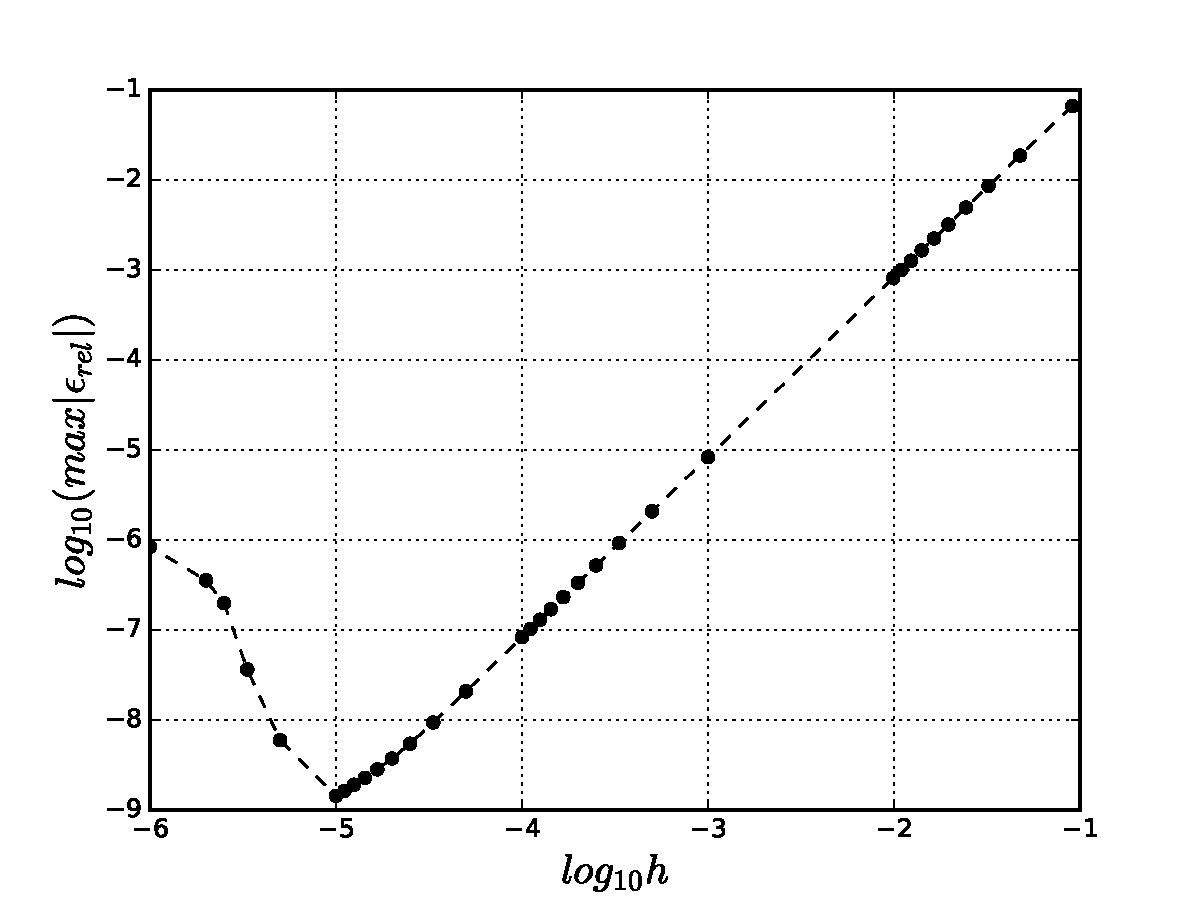
\includegraphics[scale=0.5]{relative_error_log}
    \caption{Dependency between maximum relative error and domain discretization step size on logarithmic scale. Roughly estimation of convergence rate is $2.2$. Round-off errors dominate for the small step size (less then $10^{-5}$).}
    \label{fig:error}
  \end{center}
\end{figure}

\subsection{Discussion}

\end{document}
